\chapter{The Original Uncanny Valley}
\label{chap:2}
The uncanny valley was first hypothesised by a robotics professor at the Tokyo Institute of Technology. In an essay Masahiro Mori published in 1970 \cite{original_masahiro_not_translated}, he theorised that as the appearance of a robot is approaching, but failing to attain, a lifelike appearance, the empathy of a person towards the robot would abruptly shift from affinity to revulsion.
At first, little attention was paid to his work; however, as technology evolved and more human-like robots were being built, the effects of the uncanny valley gained more significance in robotics and other scientific fields \cite{original_masahiro}.

\section{The Uncanny Valley in Terms of Appearance}
To explain the uncanny valley in more detail, Masahiro Mori \cite{original_masahiro} chose three different robots with varying human-likenesses with regard to their appearance and described people's feelings toward these robots. First, he considered an industrial robot whose design is solely based on functionality. Given their non-existent resemblance to humans and their exclusively functional existence, people feel hardly any affinity towards them.\\
Next, a toy robot with a roughly human-looking external form was examined. Especially children can get very attached to such toys. This reaction reveals that our affection for robots rises with a higher human resemblance.\\
To now show that the affinity for a robot does not increase linearly with its human similarity, Masahiro Mori explained that a prosthetic hand had achieved a near-perfect resemblance to the human form. However, as soon as a person realises that the hand is actually artificial, most people experience an eerie sensation. The loss of affinity towards the hand can be described as the uncanny valley.
In the following graph \ref{fig:uv_appearance}, where the x-axis corresponds to the human-likeness, and the y-axis corresponds to the affinity, all three examples are plotted to depict the uncanny valley. 
\begin{wrapfigure}[13]{r}{0.5\textwidth} %this figure will be at the right
    \centering
    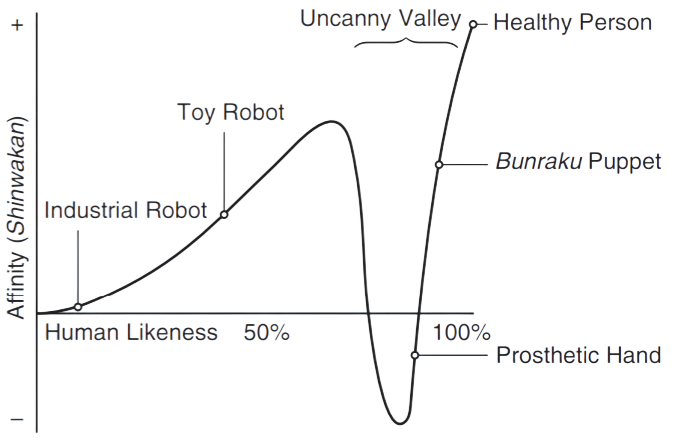
\includegraphics[width=0.5\textwidth]{graphics/uv_appearance.png}
    \caption{The uncanny valley in terms of appearance.}
    \label{fig:uv_appearance}
\end{wrapfigure}
The graph illustrates how the human-likeness at first grows linearly with regards to affinity, but at a very high, but not perfect human resemblance, the affinity falls rapidly.\\ 
Overcoming the uncanny valley is, however, possible according to Masahiro Mori's hypothesis, which can be noticed by the Bunraku Puppet entry in the graph. A Bunraku is a traditional Japanese form of musical puppet theatre, and even though it might not be more human-like than a prosthetic, on close inspection, its total appearance and movement from a distance are remarkably human-like. Masahiro Mori proposed that although they are very human-like, they are not perceived as repulsive by the audience.

\section{The Effect of Movement}
Masahiro Mori's original hypothesis \cite{original_masahiro} also factored in the effect of movement on the uncanny valley. He proposed that movement profoundly impacts the uncanny valley by amplifying the peaks and valleys seen in figure \ref{fig:uv_appearance}. This phenomenon can again be better illustrated with the example of the industrial robot and the prosthetic hand. When the industrial robot is programmed to move like a human, it feels more human-like, and we feel a higher affinity towards the robot. On the contrary, when the prosthetic hand, which already creates a robust uncanny valley effect with its appearance, starts to move, the feeling of eeriness intensifies.
Figure \ref{fig:uv_movement} illustrates how adding movement steepens the slopes of the uncanny valley.
\begin{wrapfigure}{r}{0.5\textwidth} %this figure will be at the right
    \centering
    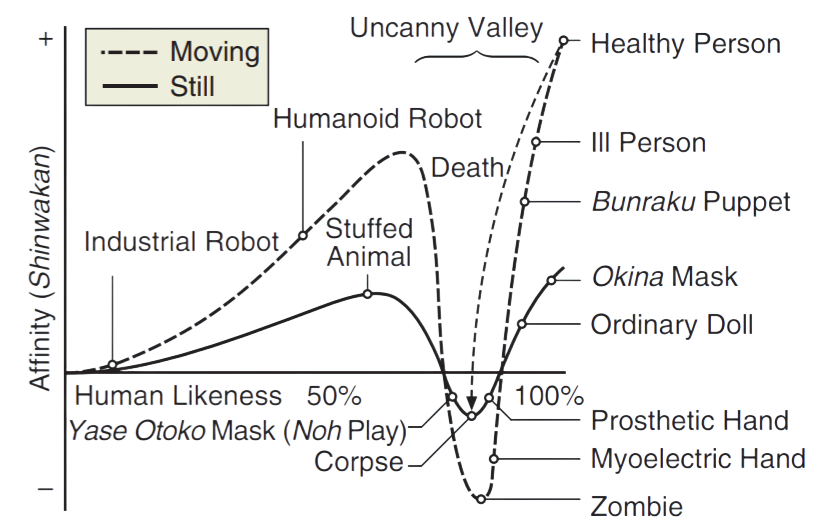
\includegraphics[width=0.5\textwidth]{graphics/uv_movement.png}
    \caption{The effect of movement on the uncanny valley.}
    \label{fig:uv_movement}
\end{wrapfigure}
Since even the movement of a single body part can have a negative effect, the unnatural movement of an entire robot can have a strong adverse effect on the affinity towards a robot. Furthermore, it is elementary for a human to recognise the slightest variations in movements which do not exactly match the human version of this movement. This can quickly lead to an entity that has come close to a human appearance falling deep into the uncanny valley. In summary, movement can amplify the slopes of the uncanny valley proposed by Masahiro Mori.